\section{Paměťové obvody}
-rozdělení pamětí, vlastnosti, typy, struktura. DRAM(1T), SRAM (6T), EEPROM, FLASH (SLC, MLC, TLC, PLC). Popište základní princip jednotlivých typů pamětí a jejich strukturu na tranzistorové úrovni

\subsection{Rozdělení pamětí}
\textbf{Podle možnosti zápisu:}\\
-RWM - Read Write Memory: paměť pro zápis i čtení, po odpojení napájení se obsah ztrácí\\
-ROM - Read Only Memory: paměť pouze pro čtení, po odpojení napájení se obsah uchovává\\

\textbf{Podle přístupu k paměti:}
-RAM - Random Acces Memory: paměť s libovolným přístupem\\
-SAM - Serial Acces Memory: paměť se sériovým pčístupem\\
-CAM - Content Acces Memory: paměť s adresovatelným obsahem\\
-FIFO - First In First Out: paměť typu první dovnitř, první ven\\
-LIFO - Last In First Out: paměť typu poslední dovnitř, první ven (zásobník)

\textbf{Podle principu realizace paměťové buňky:}\\
Statické(SRAM): buňka paměti je tvořena bistabilním klopným obvodem\\
Dynamické(DRAM): vyžadují "refresh" obnovení náboje

\textbf{Podle způsobu záznamu a mazání:}\\
ROM: programují se ve výrobě IO maskou - unipolární\\
PROM: 1x programovatelné-přetavením tavné pojistky - bipolární\\
EPROM: elektricky programovatelné - mazatelné UV zářením - unipolární\\
EEPROM: elektricky programovatelné i mazatelné - unipolární\\
FlashEPROM: verze EEPROM s velmi krátkou dobou čtení a zápisu\\
\newpage
\subsection{DRAM(1T)}
   \begin{figure}[h]
   \begin{center}
     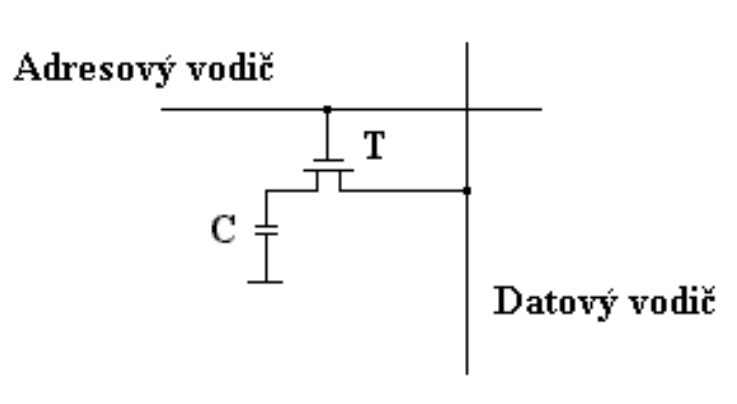
\includegraphics[scale=0.4]{images/DRAM.png}
   \end{center}
   \caption{Paměť DRAM}
  \end{figure}

\textbf{Zápis:}\\ 
Na adresový vodič se přivede hodnota logická 1. Tím se tranzistor T otevře. Na datovém vodiči je umístěna zapisovaná hodnota (např. 1). Tato hodnota projde přes otevřený tranzistor a nabije kondenzátor.  

\textbf{Čtení:}\\
Na adresový vodič je přivedena hodnota logická 1, která způsobí otevření tranzistoru T. Jestliže byl kondenzátor nabitý, zapsaná hodnota přejde na datový vodič. Tímto
čtením však dojde k vybití kondenzátoru a zničení uložené informace. Jedná se tedy o buňku, která je \textbf{destruktivní při čtení} a přečtenou hodnotu je nutné opět do paměti zapsat.

Buňka paměti DRAM je velmi jednoduchá a dovoluje vysokou integraci, a má nízké výrobní
náklady. Díky těmto vlastnostem je používána k výrobě operačních pamětí. Její nevýhodou je však vyšší přístupová doba (60 - 70 ns), způsobená nutností provádět refresh a časem potřebným k nabití a vybití kondenzátoru.

   \begin{figure}[h]
   \begin{center}
     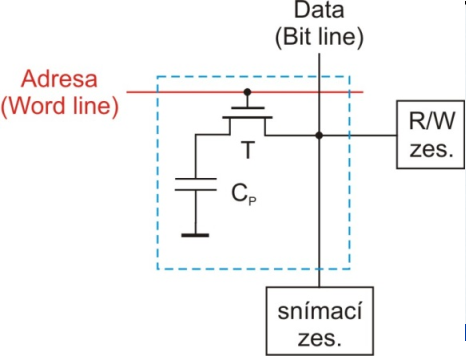
\includegraphics[scale=0.6]{images/DRAM2.png}
   \end{center}
   \caption{Paměť DRAM}
  \end{figure}
\pagebreak
\subsection{SRAM(6T)}
   \begin{figure}[h]
   \begin{center}
     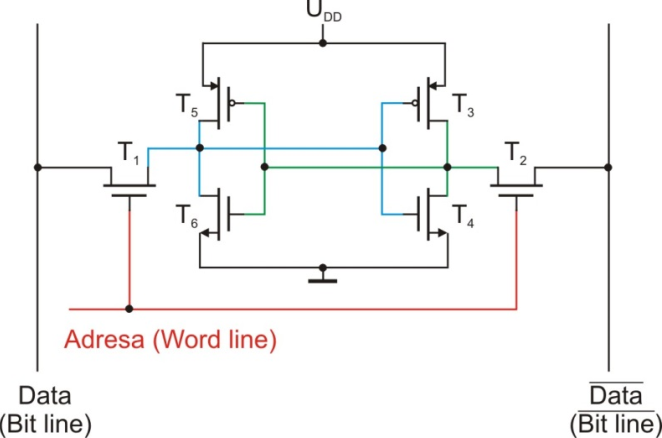
\includegraphics[scale=0.6]{images/SRAM.png}
   \end{center}
   \caption{Paměť SRAM}
  \end{figure}
\textbf{Zápis:}\\
Při zápisu se na adresový vodič umístí hodnota H. Tranzistory T1 a T2 se otevřou.
Na vodič se přivede zapisovaná hodnota (např. 1). Tranzistor T1 je otevřen, takže jednička na vodiči je přivedena na vstup invertoru tvořeného tranzistory T4 a T3.
Výstup invertoru (T4, T3) tvoří vstup invertoru tvořeného tranzistory T5 a T6. Tento stav obvodu představuje uložení hodnoty 0 do paměti. Zcela analogicky tato buňka pracuje i při zápisu hodnoty 1. Rozdíl je pouze v tom, že výstup invertoru (T4, T3) je v logické úrovni H.

\textbf{Čtení:}\\
Při čtení je opět na adresový vodič přivedena hodnota logická 1, což opět způsobí otevření tranzistorů T1 a T2. Jestliže byla v paměti zapsána hodnota 1, je na výstupu invertoru (T4, T3) hodnota 0. Tuto hodnotu obdržíme na vodiči . Opět zcela analogicky v případě uložené hodnoty 0, kdy tranzistor T4 je uzavřen (tj. na jeho výstupu je hodnota 1). 

\subsection{EEPROM}
   \begin{figure}[h]
   \begin{center}
     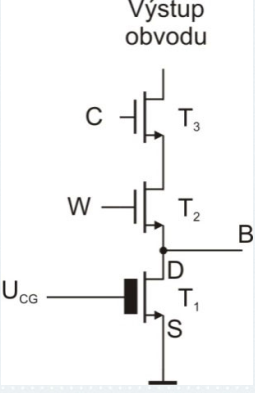
\includegraphics[scale=0.6]{images/EEPROM.png}
   \end{center}
   \caption{Paměť EEPROM}
  \end{figure}
Energeticky nezávislá polovodičovou paměť typu ROM s možností zápisu, smazání a přepisu dat.\\
Další výhodou paměťových buněk EEPROM je nejmenší velikost sektoru, kterou je možné vymazat.\\ 
Při zvýšení napětí na řídící elektrodě CG se elektrony Fowler-Nordheimovým tunelováním přenesou z D na plovoucí hradlo. Není potřeba žádný proud kanálem. Proud tunelování je relativně malý, proto nabíjení plovoucího hradla probíhá pomaleji. Při opačné orientaci elektrického pole dochází tunelováním k odstranění elektronů.

Lze mazat jednotlivé buňky (tunelováním) Počet mazacích cyklů 10\textsuperscript{4} – 10\textsuperscript{6}.
Nevýhodou je větší složitost → větší cena Při zápisu logika zajistí vymazání předchozí
informace.\\
Vzhledem k dlouhé době programování je nutná kontrola ukončení programovacího cyklu Pro zrychlení bylo zavedeno programování stránky (page write mode).

\subsection{FLASH}
Programovat lze jednotlivý byte paměti, ale mazat lze pouze celá paměť (bulk erase), případně její jeden sektor (Sektor Erase FLASH memory) nebo blok.

Jednotranzistorová buňka vychází z pamětí EPROM a využívá se tranzistor s plovoucím hradlem.
Mazání je umožněno změnou tvaru elektrody S (Source). Programování probíhá injekcí horkých elektronů z kanálu při přivedeném zvýšeném napětí na řídicím hradle. Elektrické mazání probíhá při uzemněném řídicím hradle a zvýšeném napětí na elektrodě Source, které způsobí tunelování elektronů z paměťového tranzistoru. Tranzistor se tak uvede do původního stavu. Na rozdíl od pamětí EEPROM se u pamětí flash provádí mazání nikoliv po jednotlivých buňkách, ale po celých blocích.

Novější typy obsahují nábojovou pumpu (tzn. nevyžadují zvýšené napětí 12 V). Paměť rozdělena do bloků, může obsahovat „Boot block“.

NOR a NAND flash se liší ve dvou důležitých
faktorech:
\begin{itemize}
\item Různé propojení paměťových buněk
\item Mají odlišné rozhraní pro čtení a zápis dat do paměti
\item NOR umožňuje náhodný přístup pro čtení,
\item NAND umožňuje pouze přístup ke stránce.
\end{itemize}
NAND - Byla vyvinuta s cílem snížit plochu čipu, která je potřebná k provedení dané kapacity.
Tzn. snížit náklady na kus, zvýšení maximální kapacity čipu tak, aby byla konkurence schopná se
záznamovými zařízeními, jako jsou pevné disky
\subsubsection{NOR FLASH}
NOR Flash, které poskytují rozhraní s vyhrazenými adresovými a datovými vodiči, tzn., že umožňují přímý přístup k dané paměťové buňce.\\
Chovají se jako paměti, které jsou mapované do určité části adresového prostoru. Díky tomu mají menší hustotu paměťových buněk, jsou pomalejší při zápisu,
ale mají vyšší rychlost při čtení než paměti NAND Flash.\\
Název je odvozen podle uspořádání tranzistorů, které
odpovídá struktuře hradla NOR.

\subsubsection{NAND FLASH}
NAND Flash, využívají jednoduchého připojovacího rozhraní, takže nevyžadují plnou šířku adresové a datové sběrnice. Data jsou multiplexována do osmi vstupních/výstupních linek. Práce s NAND flash pamětí probíhá typicky v následujících krocích:
\begin{itemize}
\item zaslání příkazu (např. read nebo write),
\item zaslání 4bytové adresy, vyjadřující odkud budou data
čtena, resp. kam budou zapisována,
\item vyčkání, až flash paměť umístí požadovaná data do
výstupního registru nebo zaslání zapisovaných dat,
přečtení, resp. zapsání dat
\end{itemize}
   \begin{figure}[h]
   \begin{center}
     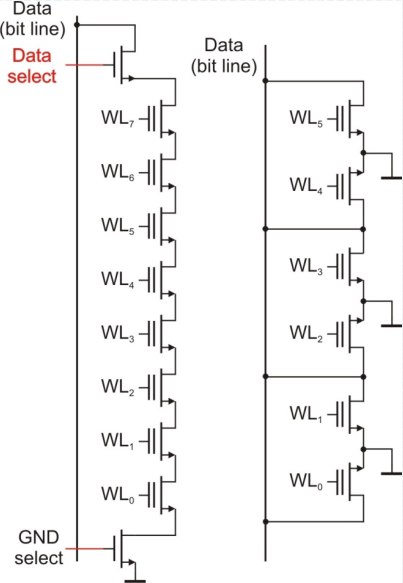
\includegraphics[scale=0.6]{images/FLASH.png}
   \end{center}
   \caption{Porovnání FLASH NAND (vlevo) a NOR (vpravo)}
  \end{figure}
  
\subsection{FLASH SLC, MLC, TLC, PLC}
\subsubsection{SLC - Single Level Cell}
Stav „1“ - buňka se nabije na 20 \%\\
Stav „0“ - buňka se nabije na 80 \%\\
Hodnoty jsou od sebe dostatečně vzdáleny\\
Životnost 100 000 přepisů\\
\subsubsection{MLC - Multi Level Cell}
Stav „11“ – buňka se nabije na 25 \%\\
Stav „10“– buňka se nabije na 45 \%\\
Stav „01“– buňka se nabije na 65 \%\\
Stav „00“– buňka se nabije na 65 \%\\
Větší pravděpodobnost vzniku chyby\\
Životnost 10 000 přepisů\\
   \begin{figure}[h]
   \begin{center}
     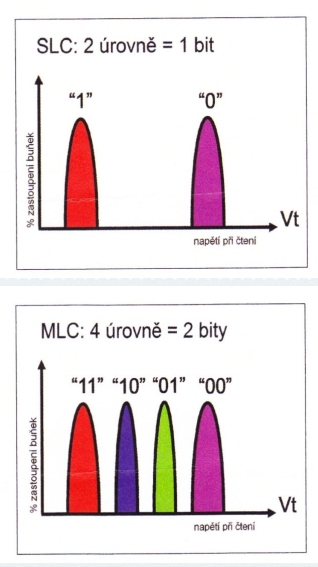
\includegraphics[scale=0.6]{images/SLC.png}
   \end{center}
   \caption{SLC a MLC FLASH paměť}
  \end{figure}
\subsubsection{TLC - Triple Level Cell}
Každý ze tří bitů dat v buňce TLC flash je buď naprogramován (0), nebo vymazán (1). Na základě úrovně napětí má paměťová buňka TLC celkem osm možných stavů: 000, 001, 010, 011, 100, 101, 110 nebo 111. Naproti tomu SLC flash má pouze dva stavy (0 nebo 1) a MLC flash má čtyři stavy (00, 01, 10, 11).  
    \begin{figure}[h]
   \begin{center}
     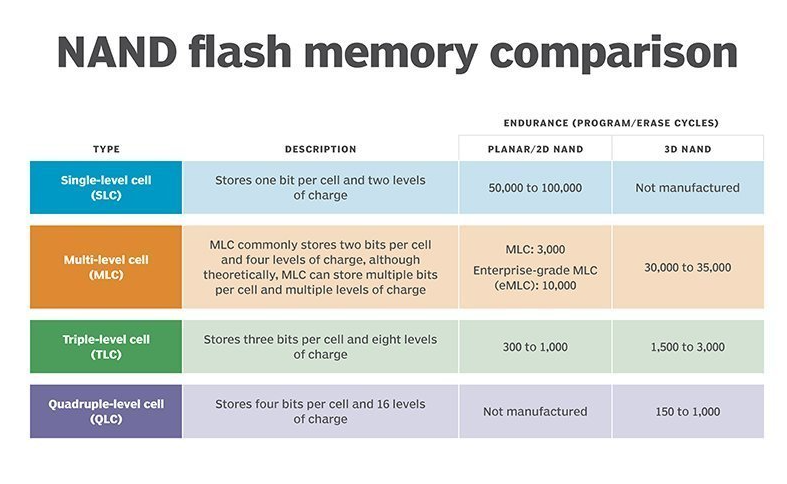
\includegraphics[scale=0.6]{images/TLC.png}
   \end{center}
   \caption{Porovnání SLC, MLC, TLC a QLC}
  \end{figure} 
\pagebreak   
\subsubsection{QLC -Quad-Level Cell}
QLC obsahují 4 bity v jedné paměťové buňce.
Konečné produkty mají ve srovnání s MLC / TLC následující výhody a nevýhody:
\begin{itemize}
\item Nižší cena za gigabajt
\item Vyšší náchylnost k opotřebení paměti a teoreticky vyšší pravděpodobnost chyb zápisu dat
\item Nižší rychlost zápisu dat
\end{itemize}
\pagebreak
\subsubsection{PLC - Penta Level Cell}
PLC obsahují 5 bitů v jedné paměťové buňce.
    \begin{figure}[h]
   \begin{center}
     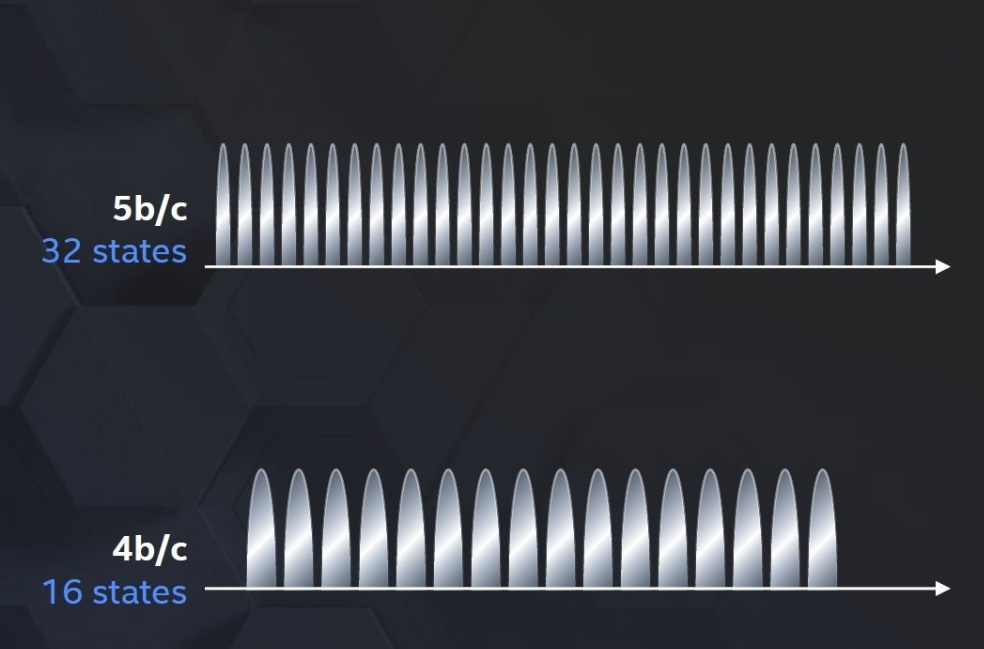
\includegraphics[scale=0.4]{images/PLC.png}
   \end{center}
   \caption{Porovnání PLC a QLC}
  \end{figure}
\newpage
\subsection{ROM}
    \begin{figure}[h]
   \begin{center}
     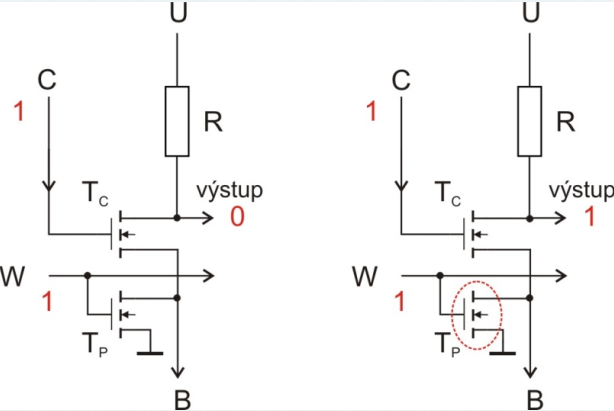
\includegraphics[scale=0.4]{images/ROM.png}
   \end{center}
   \caption{Paměť ROM}
  \end{figure}
Výběru sloupce C a řádku W, vybraný MOS paměťový tranzistor TP sepne a na
bitovém vodiči B generuje úroveň L. Tato úroveň se přes spínací tranzistor TC
přenese na výstup obvodu. Pokud nelze tranzistor TP sepnout (např. z důvodu větší vrstvy SiO2), bude na bitovém vodiči B úroveň H.
    \begin{figure}[h]
   \begin{center}
     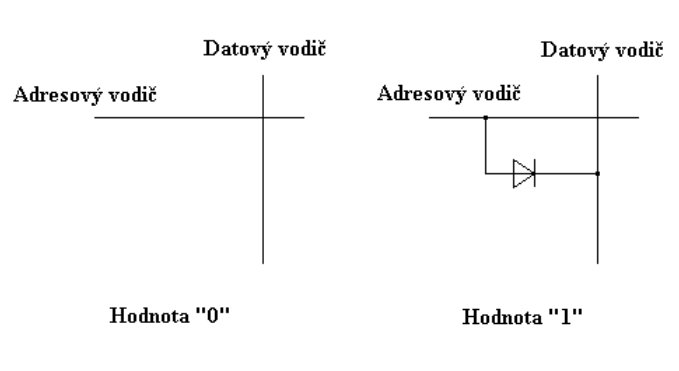
\includegraphics[scale=0.4]{images/ROM2.png}
   \end{center}
   \caption{Paměť ROM-principiálně}
  \end{figure}
  \newpage

 
\subsection{PROM}
     \begin{figure}[h]
   \begin{center}
     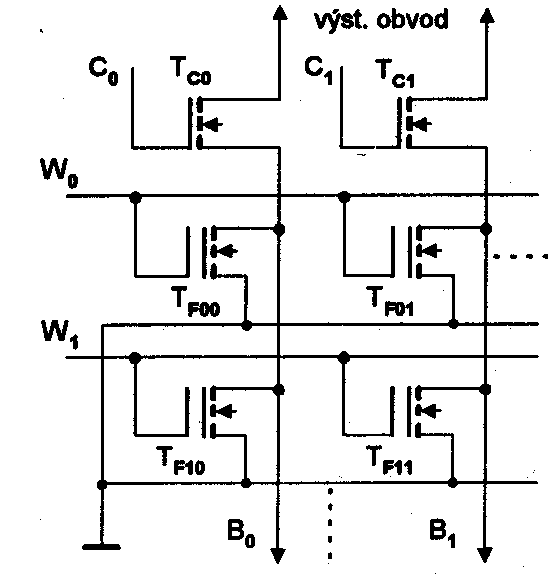
\includegraphics[scale=0.4]{images/PROM2.png}
   \end{center}
   \caption{Paměť PROM}
  \end{figure}
Alternativa k pamětem ROM, PROM nebo také OTP (anglicky One Time
Programmable) je elektricky "jednorázově" programovatelná permanentní paměť. představují statické a energeticky nezávislé paměti.
    \begin{figure}[h]
   \begin{center}
     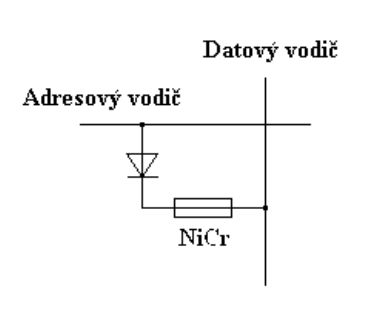
\includegraphics[scale=0.4]{images/PROM.png}
   \end{center}
   \caption{Paměť PROM - principiálně}
  \end{figure}
 \subsubsection{PROM - programování}
 Řídicí elektroda G (Gate) je připojena na vybraný adresovací
slovní vodič W se zvýšeným napětím obvykle okolo 12 V. Pokud
je na elektrodě D, která je připojena na vybraný bitový vodič B
kladné napětí (řádově okolo 5 až 6 V), protéká indukovaným
kanálem typu N od elektrody S k elektrodě D velký proud,
elektrony mají velkou energii a působením elektrického pole
mezi kanálem a řídicí elektrodou G dojde k přeskočení tzv.
horkých elektronů z kanálu přes izolační bariéru na plovoucí
hradlo, kde zůstanou. Pokud je na elektrodě D nulové napětí,
kanálem neteče proud a nedojde k přeskoku elektronů a
naprogramování paměťové buňky.

 \subsubsection{PROM - čtení}
 Při normálním režimu čtení paměťové buňky je na
elektrodě D napětí řádově 1 V a na elektrodě G ve
vybraném řádku 5 V. Přítomnost náboje na
plovoucím hradle ovlivňuje indukovaný kanál a je
potřeba větší napětí na elektrodě G (mezi 7 – 9 V),
aby kanálem protékal proud.
Toto napětí způsobí u nenaprogramovaných buněk
větší proud. Ten se vyhodnocuje jako uložený stav
H, malý proud indikuje uložený stav L.



























